\documentclass[UTF8]{ctexart}

% 设置页边距
\usepackage{geometry}
\geometry{left=2.5cm,right=3.18cm,top=2.5cm,bottom=2.54cm}

% 图片
\usepackage{graphicx}
% 图片位置
\usepackage{float}
% 并排
\usepackage{subfigure}
\usepackage{parskip}

\usepackage{lipsum}


% 由于 flushleft/right 取消了 ctex 的默认缩进
% 需要手动设置缩进
\setlength{\parindent}{2em}

% 三线表
\usepackage{booktabs}

% 设置目录显示的深度
\setcounter{tocdepth}{3}

% 设置标号深度
\setcounter{secnumdepth}{3}


\usepackage{setspace}
\date{}

\begin{document}
    % 插入校徽
	\begin{figure}[t]
		\centering
        
\includegraphics[scale=0.7]{img/HZAU.png}
	\end{figure}

	\begin{center}
		\quad \\
		\quad \\
		\heiti \fontsize{45}{17} 低脂火腿肠加工工艺及品评实验总结
		\vskip 3.5cm
		\heiti \zihao{2} 小龙虾火锅口味低脂火腿肠加工工艺研发
	\end{center}
	\vskip 3.5cm

	\begin{quotation}
		\heiti \fontsize{15}{15}
		\doublespacing
		\par\setlength\parindent{12em}
		\quad

		学\hspace{0.61cm} 院:信息学院

		专\hspace{0.61cm} 业:生物信息学

		学生姓名:张子栋

		学\hspace{0.61cm} 号:2020317210101


		\vskip 1.5cm
		\centering
        湖北~·~武汉\\
		2023 年 12 月 28 日
	\end{quotation}

	\newpage

    \tableofcontents
    
    % 目录设为页码 0(从正文起为第一页)
    \setcounter{page}{0}

    % 目录的页脚设为空
    \thispagestyle{empty}

    \newpage

	\section{前言}
	\subsection{背景与实验目的}

	近年来,随着畜牧业的发展,我国肉类生产量持续上升,肉类和肉制品成为现代食品消费不可
	或缺的一部分。中式香肠是我国传统腌腊肉制品之一,以其独特的风味深受广大消费者欢迎。
	自 20 世纪 80 年代以来,随着国外肉质品加工技术和设备的引进,广大的肉制品开发人员自发
	地开始用西式肉制品的研究方法、观点、技术、材料和仪器来研究中式肉制品,并取得了一些
	成绩。

	传统中式香肠历史悠久,是以保存食品为首要目的形成和发展起来的,随着时代发展,传统
	中式香肠的传承需要年轻人的青睐来延续,而目前传统火腿肠的口味较为单一,缺少新品种
	以及更符合年轻人口味的火腿肠,这在一定程度上限制了传统中式香肠的消费人群。

	小龙虾风味独特、肉质鲜美,是当代年轻人聚会最喜爱的食物之一。而火锅是中国独创的美
	食之一,也是一种老少皆宜的食物。火锅不仅是一种烹饪方式,更是一种文化的象征。小龙
	虾和火锅口味的火腿肠也一定会备受年轻群体喜爱。

	\subsection{实验意义}

	创新性火腿肠的制作有以下意义:
	\begin{enumerate}
		\item 满足消费者口味需求,在食品行业中,创新性火腿肠的制作有助于满足不断变
		化的消费者口味需求\textsuperscript{\cite{ref1}}。通过引入新颖的风味、
		独特的材料组合或独特的烹饪方式,能够为消费者提供更多选择,提升产品的吸引力,
		比如周黑鸭口味、小龙虾口味、川香火锅口味等。

		\item 市场竞争力,食品市场竞争激烈,创新性火腿肠可以成为企业区别于竞争对手
		的关键因素\textsuperscript{\cite{ref2}}。通过不断推陈出新,引入与众不
		同的产品,能够吸引更多消费者的目光,从而提高品牌在市场上的竞争力,比如汉堡品
		牌塔斯汀就是结合汉堡和中国菜,推出鱼香肉丝口味的汉堡包。

		\item 适应健康趋势,随着人们对健康生活方式的关注不断增加,创新性火腿肠的制
		作也可以回应这一趋势\textsuperscript{\cite{ref3}}。调整成分,减少添加剂,
		提供更健康的食品选项,能够符合当代消费者对于食品健康的追求。
		
		\item 拓展市场,引入创新性的火腿肠,不仅可以满足本地市场的需求,还可以拓展到
		其他地区和文化。通过考虑不同地域的口味偏好,可以定制具有地域特色、符合地域口味
		的产品,吸引更广泛的受众,扩大市场份额。比如在四川推广川香火锅口味火腿肠,在长
		沙推广臭豆腐口味和小龙虾口味,在武汉推广周黑鸭风味的火腿肠。
	\end{enumerate}

	综合而言,创新性火腿肠的制作不仅关乎满足消费者个性化的口味诉求,还是企业保持市场
	活力和吸引力的关键手段。

	\subsection{实验原理}


	在食材组合和配比方面,制作创新性火腿肠的第一步是选择合适的食材,包括肉类、调味料、
	添加剂等\textsuperscript{\cite{ref4}}。通过精确的配比和独特的食材组合,可以
	打造出独特口感和风味的产品。其次,采用不同的加工技术,如绞肉、搅拌、挤压等,以确保
	食材均匀混合,形成具有一致质地和口感的火腿肠。同时,使用适量的添加剂和调味料,如盐、胡椒、香辛料等,可以调整火腿
	肠的口味,延长产品的保质期,并提升整体的味觉体验\textsuperscript{\cite{ref5}}。之后,选择适当的烹饪方法,如烟
	熏、蒸煮、烤制等,对火腿肠进行加热和处理,以确保产品的风味、色泽和质地得到优化\textsuperscript{\cite{ref6}}。

	除此之外,运用先进的食品技术,如植物蛋白提取、细胞培养等,以实现更广泛的原料选择,
	提高产品的创新性和可持续性。还需要考虑市场趋势和消费者反馈,灵活调整产品配方和制作
	工艺,以适应不断变化的市场需求。这些综合运用能够促使创新性火腿肠的成功制作,创造出
	符合消费者口味偏好和市场趋势的产品。

	\begin{figure}[!htb]
		\centering
		\subfigure[研发流程]{
			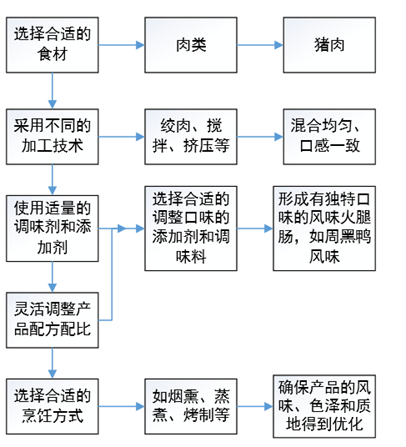
\includegraphics[scale=0.5]{img/pipeline.png}
		}
		\subfigure[火腿肠原料]{
			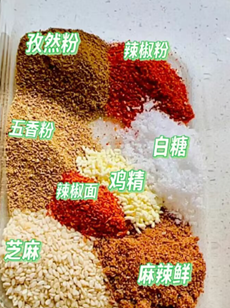
\includegraphics[scale=0.7]{img/ingredient.png}
		}
		\subfigure[火腿肠成品]{
			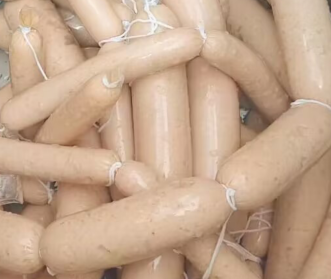
\includegraphics[scale=0.773]{img/product.png}
		}
		\caption{火腿肠研发流程(左上图 a),火腿肠制作中需要用到的原料(右上图 b),火腿肠加工后的成品(下图 c)。}
        
	\end{figure}



	\newpage

	\section{实验材料与仪器设备}
	在试验中需要用到以下仪器和材料:

	\begin{table}[!htb]
        \begin{minipage}[h]{0.36\linewidth}
            \centering
			\caption{小龙虾风味火腿肠原料配比}
                \begin{tabular}{cc}
					\toprule
					材料 & 用量\\
					\midrule
					猪肠衣	&	半包\\
					食用油	&	25~g\\
					生抽	&	25~mL\\
					老抽	&	25~mL\\
					味极鲜	&	10~mL\\
					红曲粉	&	20~kg\\
					猪肉糜	&	2.5~kg\\
					鸡蛋	&	4 个\\
					水淀粉	&	100~mL\\
					五香粉	&	50~g\\
					小龙虾肉 &	50~g\\
					小龙虾味调味粉 &	50~g\\
					\bottomrule
				\end{tabular}
        \end{minipage}
        \begin{minipage}[h]{0.36\linewidth}
            \centering
			\caption{小龙虾风味火腿肠原料配比}
			\begin{tabular}{cc}
				\toprule
				材料 & 用量\\
				\midrule
				猪肠衣	&	半包\\
				食用油	&	25~g\\
				生抽	&	10~mL\\
				老抽	&	25~mL\\
				味极鲜	&	10~mL\\
				红曲粉	&	20~kg\\
				猪肉糜	&	2.5~kg\\
				鸡蛋	&	4 个\\
				水淀粉	&	100~mL\\
				五香粉	&	50~g\\
				火锅风味调味粉 &	100~g\\
				\bottomrule
			\end{tabular}
        \end{minipage}
		\begin{minipage}{0.24\linewidth}
		\centering
        \caption{实验器材及数量}
        \begin{tabular}{cc}
            \toprule
            仪器 & 数量\\
            \midrule
            灌肠器 & 1\\
			不锈钢锅 & 3\\
			微波炉 & 1\\
			水壶 & 1\\
			棉绳 & 若干\\
			菜刀 & 1\\
			砧板 & 1\\
			蒸汽锅 & 1\\
			漏勺 & 2\\
			PE 手套 & 若干\\
			竹签 & 若干\\
			电烤肠器 & 1\\
            \bottomrule
        \end{tabular}
		\end{minipage}
    \end{table}

	注意事项:蒸汽锅需要在老师的帮助下使用,否则可能发生危险。

	其中淀粉液可以在淀粉和肉、水分结合后会让火腿肠有更好的保水性,及更好的口感,也便于灌入肠衣中;
	五香粉、生抽、味极鲜、香肠调味料等用于对火腿肠的肉馅进行调味;其中小龙虾调味粉为火腿肠增加小
	龙虾风味,小龙虾肉给火腿肠增加虾肉口感,使得口感和味道更加贴合龙虾口感。香肠调味料火锅风味给
	火腿肠具有火锅的风味,具有火锅的香气和口味,使其味觉上更加独特。红曲粉用于给火腿肠调色,增
	加视觉的诱人感,同时可以降低亚硝酸盐的食用量。天然肠衣具有质地薄韧柔软、富含胶原蛋白与弹性蛋
	白、具有良好的透气性、可食性和弹性等优点,天然肠衣的应用,不但能够保持香肠的优良风味品质,还能
	够提高香肠制品的安全性,但天然肠衣规格不统一,可能含有农兽药残留、肠道细菌和外源微生物污染等
	问题,不利于机械化和标准化生产;塑料肠衣机械强度高,具有不透水、不透气、耐腐蚀、防潮、防霉、抗
	氧化等特点,利于生产、加工和储藏,但其在遇冷后会发生皱缩、难降解,有造成环境污染的风险。

	\section{实验方法和步骤}
	\subsection{工艺条件}
	\begin{enumerate}
		\item 原料选择:选用新鲜的猪肉为主要原料,确保原料的质量符合要求。
		\item 制作工艺:制作过程包括肉切碎、加入调味料、混合搅拌、充填、煮制等环节。其中,肉肠的调味料主要包括食盐、糖、胡椒粉等,制作时应按比例加入,充填时应注意充实度和均匀度,煮制时要注意温度控制和时间。
		\item 卫生要求:制作过程中应注意卫生,要求制作场所、器具、人员、原料等各方面符合卫生标准,确保制品无菌、卫生。
		\item 贮存条件:制品成品应在冷藏、冷冻等条件下储存,并在规定的保质期内进行销售或使用,以确保产品的质量和安全性。
	\end{enumerate}

	\subsection{实验步骤}

	火锅味肉肠:

	\begin{itemize}
		\item 将绞好的肉馅化冻后剁碎放入碗中
		\item 加入盐、白糖、五香粉、姜粉、白胡椒粉、蛋清,顺着一个方向搅拌均匀
		\item 将火锅底料用水化开,放入肉馅,继续顺着一个方向搅拌
		\item 加入淀粉,再次顺着一个方向搅拌均匀
		\item 加入红曲粉,顺着一个方向搅成起胶质状态
		\item 把肉馅装进灌肠器中,挤入洗好的肠衣中,底部用绳子系紧,分成小段
		\item 水下锅大火煮开,转中小火煮40分钟捞出,放入冰水或冷水中过凉,剪成小节即可
	\end{itemize} 

	\quad

	小龙虾味肉肠:

	\begin{itemize}
		\item 将绞好的肉馅化冻后剁碎放入碗中
		\item 虾仁剁碎成泥,放入肉馅,加入盐、味精、料酒、生抽酱油、小龙虾调味料、姜末、葱末等调料,顺着一个方向搅拌均匀
		\item 加入清水,继续顺着一个方向搅拌
		\item 加入淀粉,再次顺着一个方向搅拌均匀
		\item 加入红曲粉,顺着一个方向搅成起胶质状态
		\item 把肉馅装进灌肠器中,挤入洗好的肠衣中,底部用绳子系紧,分成小段
		\item 凉水下锅大火煮开,转中小火煮40分钟捞出,放入冰水或冷水中过凉,剪成小节即可
	\end{itemize}
	\quad\\
	注意事项:
	\begin{enumerate}
		\item 肠衣在使用前需要将提前浸泡,并用水冲洗肠衣内测,确保肠衣完整不漏,去除异味。
		\item 灌肠时把肉泥填到八分满,不要用力过大,肠衣容易撑破。
		\item 做好的肠需要用牙签在表面扎几个眼方便排气,防止煮的过程中膨胀炸开。
		\item 肉肠下锅煮后产生的浮沫需要及时去除,不然会粘在肠的表面影响味道。
		\item 肉肠的味道可以自行改良,添加符合自己口味的配料。
	\end{enumerate}

	\section{结果与分析}
	\subsection{口味创新性}
	火锅味火腿肠:将火锅的香辣味融入火腿肠中,不仅可以满足喜欢火锅的人群,还能为传统火腿
	肠带来新的口感体验。这种口味对于年轻人和寻求新奇食品的消费者具有很强的吸引力。

	小龙虾味火腿肠:小龙虾是夏季热销的食品,将其味道融入火腿肠中,不仅可以满足消费者在夏
	季对小龙虾的需求,还能为火腿肠带来新的销售高峰。

	\subsection{市场可行性}
	火锅味火腿肠:目前市场上的辣味食品越来越受欢迎,火锅作为深受人们喜爱的美食之一,其味
	道具有广泛的群众基础。因此,火锅味火腿肠有可能成为新的市场热点。

	小龙虾味火腿肠:随着小龙虾市场的不断扩大,各种与小龙虾相关的食品风味食品出现在市场上
	,包括小龙虾味的薯片、拌面和泡面等等,小龙虾味火腿肠的市场潜力较大。

	\subsection{总结}
	从上述分析来看,制作火锅味和小龙虾味的火腿肠具有很高的可行性。这两种口味都是市场上较
	为新颖、独特的产品,有望为传统的火腿肠市场注入新的活力。同时,这两种口味也具有一定的
	市场基础,可以吸引更多消费者的关注和购买。

	\section{包装设计}

	外包装的颜色和图案可以清晰的展示火腿肠的口味和成分,其外形也能吸引更多的顾客购买品尝。

	\begin{figure}[htb]
		\centering
		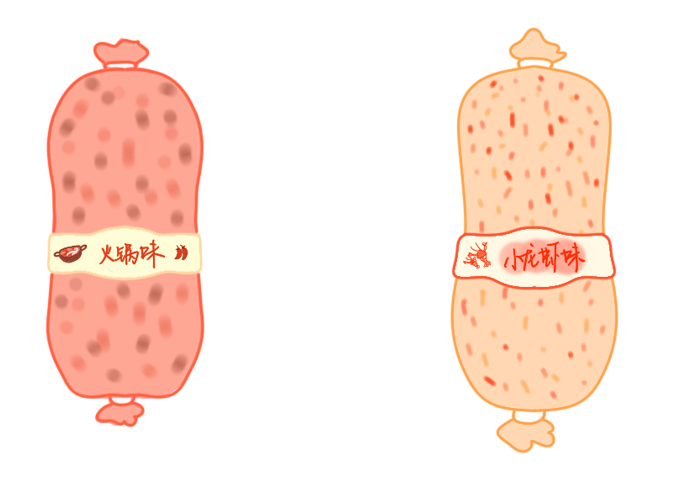
\includegraphics[width=0.5\linewidth]{img/package.png}
		\caption{火腿肠外包装}
	\end{figure}
	\section{商业背景调查}
	\subsection{行业概述}
	淀粉肠作为一种健康食品,近年来在全球范围内逐渐受到消费者的青睐。随着人们健康意识的提
	高,对于食品的选择更加注重营养与健康,淀粉肠正符合这一消费趋势。并且与其他肠类食品相
	比,淀粉肠在口感和营养价值上都有一定的优势,可以满足消费者的不同需求,具有一定的差异
	化竞争优势。中式口味淀粉肠在传统淀粉肠的基础上,引入了更多的中式调味料和食材,使得口
	感更加丰富和多元,例如火锅风味淀粉肠和小龙虾口味淀粉肠,中式口味淀粉肠更能满足现代消
	费者的口味需求,在传统形式上加以创新,更能吸引年轻消费群体。

	\subsection{市场规模与增长趋势}
	随着人们健康意识的提高和对营养均衡的需求不断增加,淀粉肠作为一种健康、美味的食品,市
	场需求量大,市场前景广阔。中式口味淀粉肠可以搭配其他食材或调料进行创新,制作出多种口
	味和特色,吸引更多消费者。因此,中式口味淀粉肠在商业上具有很大的发展潜力。据统计,全
	球低脂淀粉肠市场规模在近年来呈现出稳步增长的趋势。预计未来几年,全球低脂淀粉肠市场规
	模将继续保持增长态势。

	\subsection{中国市场分析}
	中国作为世界上最大的食品市场之一,淀粉肠市场同样庞大。国内主要生产商在淀粉肠市场上占
	据一定的份额,同时国际品牌也在积极进入中国市场。中国淀粉肠市场的竞争格局正在逐步形成,
	企业在产品质量、品牌形象和营销策略等方面需要不断创新以获得竞争优势。
	
	\subsection{产品类型分析}
	低脂淀粉肠根据产品类型和应用领域可以分为多种细分市场。家庭消费和餐饮业是主要的应用领
	域。不同类型和应用领域的低脂淀粉肠在市场规模和增长趋势方面存在差异,企业需要针对不同
	的细分市场制定相应的生产和销售策略。中式淀粉肠具有浓郁的地方特色,让消费者在享用淀粉
	肠美味口感时,也能体验中华美食的独到之处,感受中华文化的奇妙魅力。例如市面上已经批量
	生产的周黑鸭口味淀粉肠就是在传统淀粉肠的基础上,结合周黑鸭的口味特点,开发出的一种新
	型淀粉肠。它以鸭肉为主要原料,经过腌制、搅拌、灌装、烤制等工序制作而成,口感鲜美、香
	辣可口,深受消费者喜爱。随着消费者对口味和品质的要求不断提高,传统淀粉肠已经不能满足
	市场需求。中式口味淀粉肠的推出,满足了消费者对于新口味、高品质的需求,具有很大的市场
	潜力。

	\subsection{产业链分析}
	低脂淀粉肠的产业链包括上游原料供应商、中游生产商和下游销售渠道。上游供应商主要为生产
	提供原料和设备,中游生产商负责生产和加工低脂淀粉肠,下游销售渠道则通过各种方式将产品
	传递给消费者。产业链的各个环节需要协同合作,确保产品质量和供应稳定。企业需要与供应商
	建立良好的合作关系,同时加强生产和质量管理,优化销售渠道以提升市场份额。

	\section{可行性分析}
	\subsection{市场可行性}
	\subsubsection{行业概况}
	火腿肠是以畜禽肉为主要原料,辅以淀粉、植物蛋白粉等填充剂,再加入食盐、糖、酒、味精、
	香辛料等调味品,并添加品质改良剂卡拉胶和维生素C,以及护色剂、保水剂、防腐剂等物质。
	火腿肠含有供给人体需要的蛋白质、脂肪、碳水化合物、各种矿物质和维生素等营养,还具有吸
	收率高、适口性好、饱腹性强等优点,还适合加工成多种佳肴。低脂火腿肠以其低脂肪、高蛋白
	质和美味口感而备受消费者青睐。它通常由猪肉、牛肉或鸡肉等肉类加工而成,其中的脂肪含量
	通常比传统火腿肠低。这使得低脂火腿肠成为追求健康生活方式的消费者的首选之一。

	\begin{figure}[htb]
		\centering
		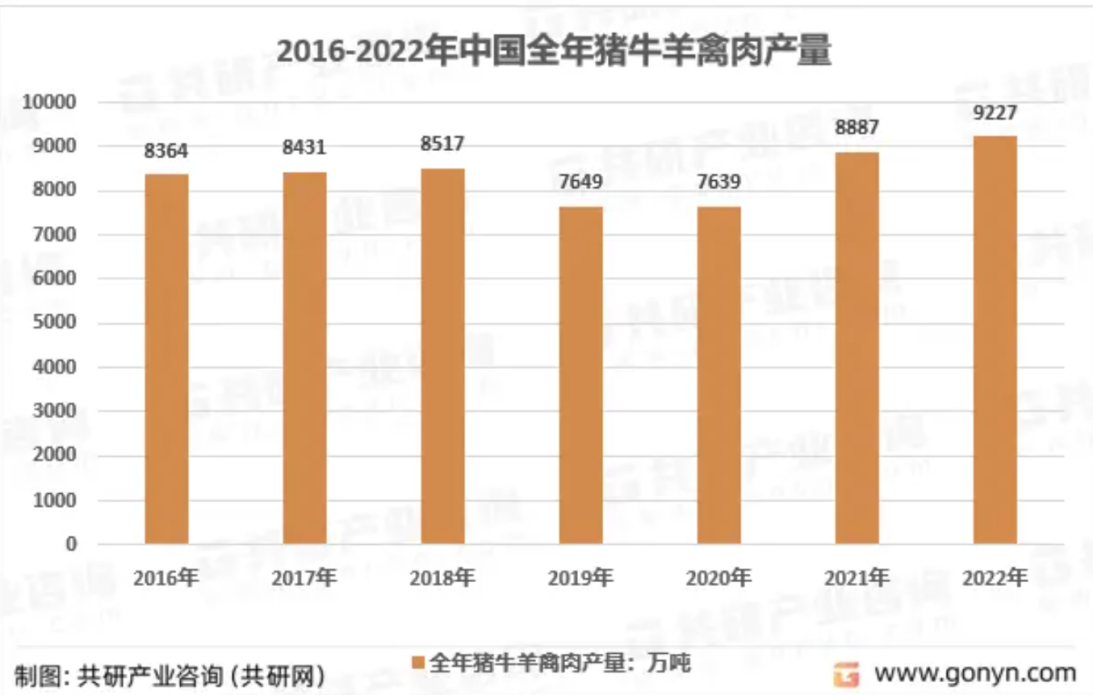
\includegraphics[scale=0.8]{img/amount.png}
		\caption{2016 - 2022 年中国全年猪牛羊禽肉产量}
	\end{figure}

	我国是肉类生产和消费大国,肉类行业已逐步成为关系到国计民生的重要产业。据统计,2021年,
	全年猪牛羊禽肉产量 8887 万吨,比上年同期增长 16.34\%。国家统计局最新数据显示,2022年全
	年我国猪牛羊禽肉产量 9227 万吨,比上年增长 3.8\%。火腿肠以其方便、美味、保质期长等优点,
	必将依旧成为中国近阶段肉制品的主导产品。受益于市场需求的增长,我国火腿肠产量不断增加,2023
	年我国火腿肠产量可达412.2吨。

	总体而言,在我国,火腿肠行业仍处于正在发展阶段,进五年以来,我国火腿肠的产量仍在稳步上升。
	
	\begin{figure}[htb]
		\centering
		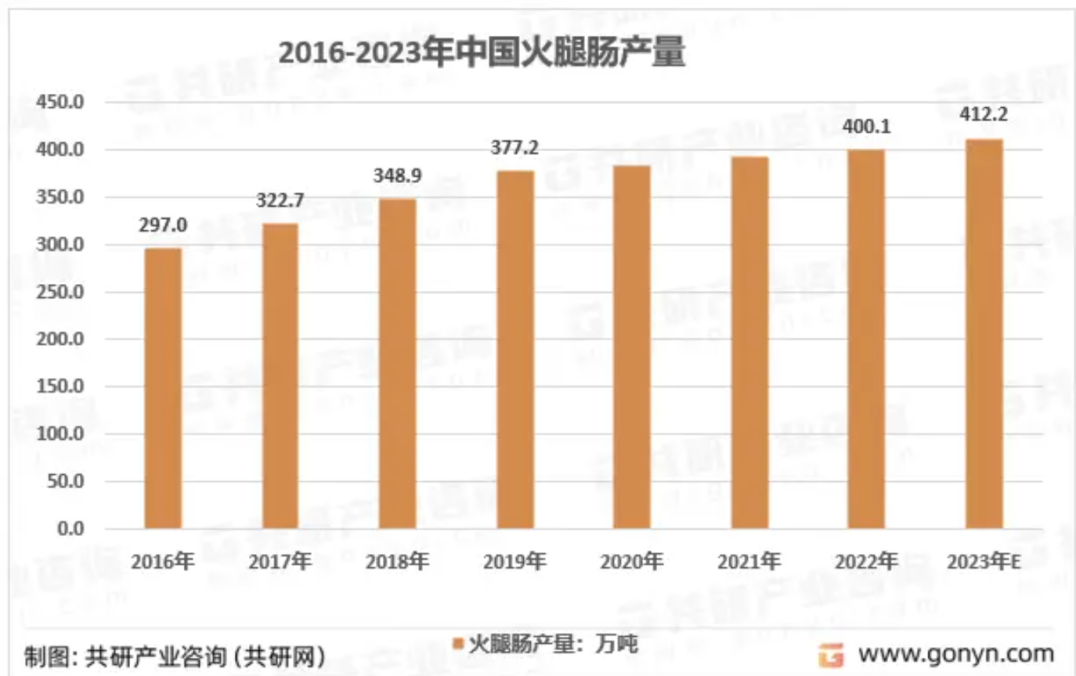
\includegraphics[scale=0.8]{img/sus_amount.png}
		\caption{2016 - 2023 年中国火腿肠产量}
	\end{figure}

	\subsubsection{市场需求}
	目前,全球市场对于低脂火腿肠的需求正在逐渐增加,尤其是在发达国家和地区,这是因为人们对膳
	食健康和营养价值的关注不断提升。此外,随着素食主义、纯素主义等饮食潮流的兴起,一些以植物
	为基础原料生产的低脂火腿肠也开始走俏市场。

	低脂火腿肠作为火腿肠界的新兴产品,这是因为现代消费者对健康和营养日益重视。低脂火腿肠通常
	含有较少的脂肪和热量,适合健康生活方式的人群。市场需求方面,消费者对低脂产品的需求不断增
	长,尤其是那些注重健康饮食、追求美食口感的消费者。此外,随着肥胖和心血管疾病等健康问题日
	益引起社会关注,越来越多的人开始选择低脂食品来维持健康状态,这也推动了低脂肉制品的市场需
	求。

	\subsubsection{行业特征}
	随着肉类加工企业的发展和壮大以及消费者需求的变化,我国火腿肠市场呈现出以下几方面特征:
	首先是品牌形象差异明显。火腿肠市场经历了导入时期——「春都」一个品牌独步天下,到多个品牌火
	腿肠纷纷涌入市场,再到后来的诸侯争霸。那么消费者是怎么看这些火腿肠品牌的呢?调查数据显
	示,消费者对春都、双汇火腿肠品牌形象的评价较高,其它品牌与之相比存在一定差距。其次是火
	腿肠在总体质量上存在较为显著差异。火腿肠消费年龄多在18-34岁之间、女性且高学历者居多。
	在对全国火腿肠消费者调查中发现,女性消费者的比例要远高于男性,男性:女性=37:63.
	
	综上所述,根据火腿肠行业的市场概况、市场特征、市场需求方面的了解,火腿肠市场虽然将近饱
	和,但是仍存在大量的需求量,并且对高质量,特点鲜明,具有良好品牌形象的火腿肠仍旧十分欢
	迎,存在一定的受众。所以,低脂火腿肠作为一种专门品类的火腿肠推向市场,极具可行性。

	\subsection{生产可行性}
	众多火腿肠品牌失去民心的主要原因是其未能依据市场变化提高产品质量标准,增加花色品种,更
	没有国家级或更高标准来更新换代,却将本来就不高的标准又降低了,火腿肠标准从开始到现在一
	直引用食品卫生国家标准中的GB2725.1肉灌肠类卫生标准。该标准规定细菌总数出厂$\le 2$万个,销
	售$\le 5$万个/g(未修订前分别为$3$万个/g和$5$万个/g)。火腿肠保质期为4个月(原来为6个月),温
	度要求$\le 25~℃$常温\textsuperscript{\cite{ref8}}。

	\subsection{经济可行性}
	\subsubsection{成本核算}
	
	产品生产所需所有项目及费用如下:
	\begin{table}[htb]
		\centering
			\caption{产品生产所需项目及费用(价格来自 1688 平台)}
			\begin{tabular}{ccc}
				\toprule
				原料 & 数量 & 价格\\
				\midrule
				猪肠衣 & 3.5米$/$袋(可灌5斤) & 8元\\
				食用油 & 900~mL & 14.6 元\\
				生抽 & 500~mL & 5 元\\
				老抽 & 500~mL & 6 元\\
				味极鲜 & 280~mL & 6.46 元\\
				红曲粉 & 454~g & 7.5 元\\
				猪肉 & 500~g & 11.54 元\\
				鸡蛋 & 1 个 & 1 元\\
				小龙虾肉 & 500~g & 36 元\\
				小龙虾味调味粉 & 1~袋 & 8.9 元\\
				火锅味调味粉 & 200~g/袋$\times$40 包 & 6.49 元\\		
				\bottomrule
			\end{tabular}
	\end{table}
	
	\subsubsection{目标群体}
	低脂火腿肠通常是面向关注健康饮食和体重管理的个体。这可能包括想要控制胆固醇和脂肪摄入的
	人群,以及关注心血管健康和整体身体健康的人群。另外,也有可能是为了满足儿童或家庭成员的
	膳食需求而选择低脂火腿肠。根据上述市场统计,低脂火腿肠也较受女性群体欢迎。总之,这种产
	品的目标消费群体通常包括那些注重饮食平衡和健康生活方式的人们。

	综上所述,低脂火腿肠制作成本低廉,且受众群体体量极大,具有可观的利润空间,经济意义上可
	行。低脂火腿肠基本满足市场、生产、经济可行。


	\section{感受与体会}

		在本学期的创新性实验课中,我选择了低脂火腿肠加工工艺及品评这门课。这个课题的目的
		是为了满足消费者对于火腿肠口味的多样化和健康化的需求,通过引入新颖的风味和独特的
		材料组合,创造出符合市场趋势和消费者口味的产品。在实验过程中,我学习了火腿肠的制
		作原理和方法,掌握了火腿肠的原料选择、配比、加工技术、烹饪方法等关键环节,还了解
		了火腿肠的市场分析和可行性分析,为我的实验提供了理论和数据支撑。在实验中,我遇到
		了一些困难和挑战,例如如何保证火腿肠的质量和安全性、如何调整火腿肠的口感和色泽、
		如何优化火腿肠的包装设计等,但是通过不断的尝试和改进,我最终成功地制作出了原味和
		麻辣口味的火腿肠,并对其进行了品评,得到了老师和组员一致认可。

		通过这次实验,我收获了很多。我提高了我的动手能力和创新能力,学会了运用所学
		的知识和技能来解决实际问题,开发出具有创新性和市场潜力的产品。其次,我增强了我的
		团队协作能力和沟通能力,学会了与同学和老师进行有效的交流和合作,共同完成实验任务。
		最后,我拓宽了我的视野和思维,学习了火腿肠行业的发展现状和趋势,了解了消费者的需
		求和喜好,为今后的学习和工作打下了坚实的基础。

		这次创新性实验课是一次非常有意义和有价值的学习经历,让我在实践中学习,在学习中实
		践,提升了我的综合素质和能力,也激发了我的学习兴趣和创新热情。我感谢老师和同学们
		的指导和帮助,也希望能够在今后的学习中继续努力,探索更多的知识和领域,创造更多的
		价值和贡献。

	\section*{任务分工}
	\begin{itemize}
		\item 前言
			\begin{itemize}
				\item 背景、实验目的:张城祥
				\item 实验意义、实验原理:段苏格
			\end{itemize}
		\item 实验材料与仪器设备:谢严锋
		\item 实验方法和步骤:赵若禹
		\item 结果与分析
			\begin{itemize}
				\item 产品图表:王蕾
				\item 数据分析与讨论:王源清
			\end{itemize}
		\item 包装设计:张文妍
		\item 商业背景调查:许文博
		\item 可行性分析:王思捷
		\item 报告整合与排版:张子栋
		\item PPT 汇总及汇报:尹馨唯
	\end{itemize}

	\begin{thebibliography}{99}
		\bibitem{ref1} 徐衍胜, 王福红. 素肉火腿肠的制作[J]. 肉类工业, 2020, (12):4-6.

		\bibitem{ref2} 任倩, 张诗琪, 雷激. 低温猪肉火腿肠加工工艺 [J]. 食品与发酵
		业, 2019, 45(02):166-173.DOI:10.13995/j.cnki.11-1802/ts.017355  

		\bibitem{ref3} 袁书林. 黑米弹力火腿肠的制作方法[J]. 农村百事通, 2019, (16): 42-43. DOI:10.19433/j.cnki.1006-9119.2019.16.018

		\bibitem{ref4} 李新华, 曹雪妍. 火腿肠主要配料配方的优化研究[J]. 沈阳农业大学学报, 2015, 46 (02):173-180.  

		\bibitem{ref5} 陈彦冰, 胡红梅, 孙大地, 黄从进, 刘明, 祝恒前. 鱼肉风味淀粉肠的制作和优化研究 [J]. 肉类工业, 2012, (06):5-7.   
		
		\bibitem{ref6} 程伟峰. 肉香特征香料对猪肉火腿肠风味的影响 [D]. 导师:彭增起. 南京农业大学, 2010. 
 
		\bibitem{ref7} 韩冰, 徐英楠, 侯晨, 姜晓涵, 遇世友, 李紫硕, 韩雪琪, 张根生. 肠衣制备及其对香肠品质的影响研究进展[J]. 食品安全质量检测学报, 2022, 13 (21): 7057-7064.

		\bibitem{ref8} 朱本志. 火腿肠发展方向探讨[J]. 肉类工业, 1999(05):47-48.
		
	\end{thebibliography}

\end{document}

